\documentclass[11pt]{article}
\usepackage[utf8]{inputenc}
\usepackage[spanish]{babel}
\usepackage{graphicx}         % Para incluir imágenes
\usepackage{amsmath}          % Para notación matemática
\usepackage{amsfonts}
\usepackage[margin=3cm]{geometry}  % Márgenes
\usepackage[font=normalsize,labelfont=small]{caption}  % Estilo de captions
\usepackage{hyperref}         % Para links clickeables
\usepackage{xcolor}           % Para colores en texto
\usepackage{float}            % Para usar [H] en figuras
\usepackage{booktabs}         % Para mejorar tablas (\midrule, \toprule, etc.)

% EXTENSIÓN MÁXIMA: 10 HOJAS SIN EXCEPCIÓN.
\begin{document}

\begin{titlepage}
    \centering
    \vspace*{2cm}
    
\includegraphics[scale=1.8]{figures/Logo-udesa.png}\par
    \vspace{10pt}

    {\LARGE \textbf{I302 - Aprendizaje Automático\\ y Aprendizaje Profundo}\par}
    \vspace{1cm}

    {\LARGE \textbf{Trabajo Práctico 4: \\Aprendizaje No-Supervisado}\par}
    \vspace{4cm}
    
    {\LARGE {Ilan Nomberg}\par {Ingeniería en Inteligencia Artificial}}  % <- Modificar Nombre y Apellido
    \vspace{4cm}
    
    % {\Large \today\par}
    \vspace{1cm}
    \Large{}
    \date{}
\end{titlepage}

% RESUMEN
\begin{abstract}
En este trabajo se abordaron dos tareas fundamentales de aprendizaje no supervisado: el agrupamiento de datos y la reducción de dimensionalidad. Para el primer caso, se aplicaron los algoritmos K-means, Gaussian Mixture Models (GMM) y DBSCAN sobre un conjunto bidimensional, evaluando visualmente las particiones obtenidas y utilizando métricas internas para determinar la calidad de los agrupamientos. Entre los tres enfoques, DBSCAN fue el que logró una segmentación más coherente con la estructura natural de los datos, identificando regiones densas y aislando correctamente el ruido.

En cuanto a la reducción de dimensionalidad, se trabajó sobre el conjunto MNIST, utilizando análisis de componentes principales (PCA) y autoencoders variacionales (VAE). Ambos métodos fueron evaluados en función del error de reconstrucción de las imágenes originales. Los resultados muestran que el VAE logró reconstrucciones de mayor calidad, preservando mejor los rasgos característicos de los dígitos incluso con una cantidad reducida de dimensiones latentes.
\end{abstract}

\section{Introducción}

El aprendizaje no supervisado se ocupa del análisis de datos sin etiquetas, con el objetivo de descubrir estructuras subyacentes que permitan organizar, resumir o interpretar los datos de forma automática. En este trabajo se abordan dos problemas centrales de esta área: el \textit{clustering} y la \textit{reducción de dimensionalidad}.

En primer lugar, se analiza un conjunto de datos bidimensionales mediante tres algoritmos de agrupamiento: K-means, Gaussian Mixture Models (GMM) y DBSCAN. Estos métodos permiten segmentar el espacio en regiones de alta coherencia interna, evaluando diferentes nociones de proximidad y densidad. Se explora el efecto de los parámetros clave de cada algoritmo y se comparan los resultados obtenidos mediante visualizaciones y métricas internas de calidad.

En segundo lugar, se trabaja sobre el conjunto MNIST, compuesto por imágenes de dígitos manuscritos representadas como vectores en $\mathbb{R}^{784}$. El objetivo es obtener representaciones comprimidas que conserven la mayor cantidad posible de información. Para ello, se implementan dos técnicas complementarias: análisis de componentes principales (PCA), basado en transformaciones lineales, y autoencoders variacionales (VAE), que utilizan modelos generativos no lineales entrenados mediante redes neuronales. Se evalúa la capacidad de reconstrucción de cada técnica y se comparan las representaciones resultantes.

Este enfoque combinado permite ilustrar distintas estrategias para abordar el análisis no supervisado, destacando sus aplicaciones, limitaciones y diferencias conceptuales.


\section{Métodos}
\subsection*{Clustering}

\paragraph{K-means.} Dado un conjunto de datos $\{x_1, \dots, x_n\} \subset \mathbb{R}^d$, el algoritmo K-means busca particionar los puntos en $K$ grupos disjuntos $C_1, \dots, C_K$ minimizando la suma de distancias cuadradas a los centroides:

\[
L = \sum_{k=1}^{K} \sum_{x_i \in C_k} \|x_i - \mu_k\|^2
\]

donde $\mu_k = \frac{1}{|C_k|} \sum_{x_i \in C_k} x_i$ es el centroide del cluster $C_k$. El algoritmo alterna entre dos pasos: (1) asignar cada punto al cluster más cercano, y (2) actualizar los centroides. La convergencia se alcanza cuando las asignaciones no cambian o se cumple un criterio de parada.

\paragraph{Gaussian Mixture Models (GMM).} Este modelo asume que los datos fueron generados por una mezcla de $K$ distribuciones gaussianas multivariadas:

\[
p(x) = \sum_{k=1}^{K} \pi_k \, \mathcal{N}(x \mid \mu_k, \Sigma_k)
\]

donde $\pi_k$ son los pesos de mezcla ($\sum_k \pi_k = 1$), $\mu_k$ es la media del componente $k$ y $\Sigma_k$ su matriz de covarianza. Los parámetros se ajustan mediante el algoritmo de Expectation-Maximization (EM), que alterna entre:

\begin{itemize}
    \item \textbf{E-step:} calcular las responsabilidades
    \[
    \gamma_{ik} = \frac{\pi_k \, \mathcal{N}(x_i \mid \mu_k, \Sigma_k)}{\sum_{j=1}^{K} \pi_j \, \mathcal{N}(x_i \mid \mu_j, \Sigma_j)}
    \]
    \item \textbf{M-step:} actualizar parámetros
    \[
    N_k = \sum_{i=1}^{n} \gamma_{ik}, \quad
    \mu_k = \frac{1}{N_k} \sum_{i=1}^{n} \gamma_{ik} x_i, \quad
    \Sigma_k = \frac{1}{N_k} \sum_{i=1}^{n} \gamma_{ik} (x_i - \mu_k)(x_i - \mu_k)^\top, \quad
    \pi_k = \frac{N_k}{n}
    \]
\end{itemize}

\paragraph{DBSCAN.} El algoritmo DBSCAN agrupa puntos en función de su densidad local. Dados los parámetros $\varepsilon > 0$ (radio) y $MinPts$ (mínimo de vecinos), un punto $x$ se clasifica como:

\begin{itemize}
    \item \textit{Núcleo:} si $|\mathcal{N}_\varepsilon(x)| \geq MinPts$, donde $\mathcal{N}_\varepsilon(x) = \{y : \|y - x\| \leq \varepsilon\}$.
    \item \textit{Alcanzable por densidad:} si pertenece al vecindario de un punto núcleo.
    \item \textit{Ruido:} si no es alcanzable por densidad desde ningún núcleo.
\end{itemize}

El algoritmo construye clusters conectando puntos alcanzables por densidad a partir de los núcleos. No requiere especificar la cantidad de clusters y es robusto al ruido.

\subsection*{Reducción de dimensionalidad}

\paragraph{Principal Component Analysis (PCA).} Dado un conjunto centrado de datos $X \in \mathbb{R}^{n \times d}$, PCA busca encontrar una base ortonormal $\{w_1, \dots, w_m\}$ con $m < d$ que maximice la varianza proyectada:

\[
\max_{w \in \mathbb{R}^d, \|w\| = 1} \mathrm{Var}(Xw) = w^\top \Sigma w
\]

donde $\Sigma = \frac{1}{n} X^\top X$ es la matriz de covarianza. Las componentes principales corresponden a los vectores propios de $\Sigma$ con mayor autovalor. Dado un vector $x$, su proyección y reconstrucción son:

\[
z = W^\top x, \quad \hat{x} = W z = W W^\top x
\]

donde $W = [w_1 \dots w_m]$.

\paragraph{Variational Autoencoder (VAE).} Un VAE modela la distribución de los datos como $p(x) = \int p(x \mid z) p(z) \, dz$, donde $z$ es una variable latente. Se entrena maximizando una cota inferior de evidencia (ELBO):

\[
\mathcal{L}(x) = \mathbb{E}_{q(z \mid x)}[\log p(x \mid z)] - \mathrm{KL}(q(z \mid x) \| p(z))
\]

donde $q(z \mid x)$ es la distribución aproximada (encoder), $p(x \mid z)$ es el decodificador, y $p(z)$ es un prior estándar $\mathcal{N}(0, I)$. Se asume $q(z \mid x) = \mathcal{N}(\mu(x), \sigma^2(x) I)$, y se utiliza la técnica de reparametrización para permitir el entrenamiento por gradiente:

\[
z = \mu(x) + \sigma(x) \odot \epsilon, \quad \epsilon \sim \mathcal{N}(0, I)
\]

La red se entrena minimizando $-\mathcal{L}(x)$ sobre un conjunto de datos normalizado, dividido en entrenamiento y validación.


\section{Resultados}
\subsection*{K-means}

Para aplicar K-means se evaluó la calidad del agrupamiento en función de la cantidad de clusters $K$, utilizando como métrica la suma de distancias cuadradas intra-cluster. 

Se construyó la curva de $L$ en función de $K$ para valores entre $K=1$ y $K=20$, y se utilizó una estrategia automática para seleccionar el valor óptimo de $K$ basada en el criterio de “ganancias decrecientes”. En particular, se definió un \textbf{umbral de mejora relativa} y un \textbf{parámetro de paciencia}: si la mejora relativa entre iteraciones sucesivas caía por debajo del umbral durante un número consecutivo de pasos igual a la paciencia, se detenía la búsqueda y se tomaba como $K$ óptimo el valor correspondiente a la última mejora significativa.

Este procedimiento permitió automatizar la detección del “codo” en la curva. En la Figura~\ref{fig:kmeans_elbow_auto} se muestra la evolución de $L(K)$ junto con el punto seleccionado. En este caso, el valor óptimo resultó ser $K = 15$.

\begin{figure}[H]
    \centering
    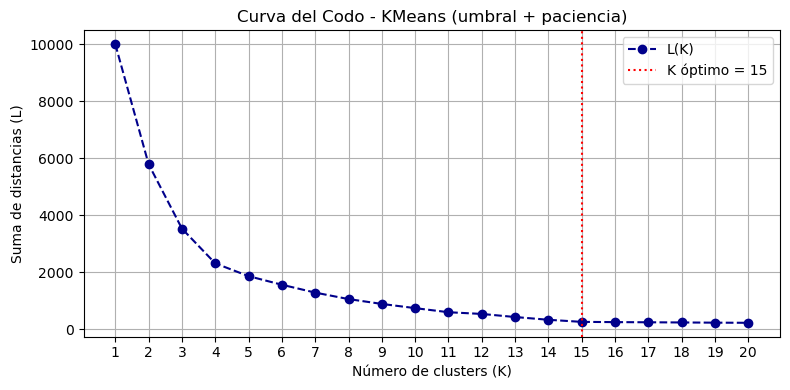
\includegraphics[width=0.6\textwidth]{figures/kmeans_elbow_threshold.png}
    \caption{Curva del codo para K-means. Se utilizó un umbral de mejora relativa y paciencia para determinar $K$ automáticamente. El valor seleccionado fue $K = 15$.}
    \label{fig:kmeans_elbow_auto}
\end{figure}

Una vez fijado el valor de $K$, se aplicó el algoritmo K-means final con múltiples inicializaciones y se seleccionó la partición que minimizaba la función de costo $L$. En la Figura~\ref{fig:kmeans_clusters_15} se visualizan los clusters obtenidos para $K = 15$, junto con sus centroides marcados como cruces negras.

\begin{figure}[h]
    \centering
    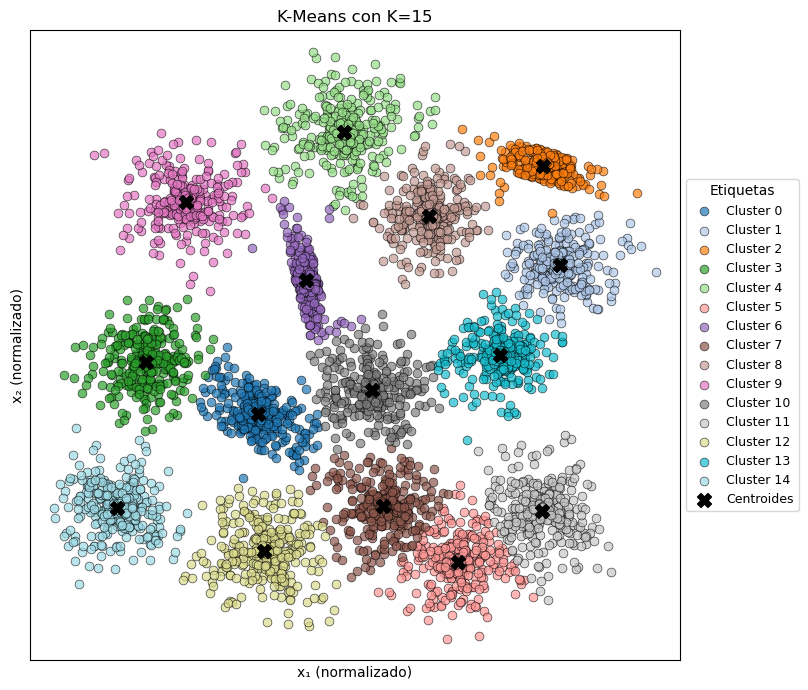
\includegraphics[width=0.6\textwidth]{figures/kmeans_clusters_k15.png}
    \caption{Clusters obtenidos mediante K-means con $K = 15$. Cada color representa un grupo distinto, y las cruces negras indican los centroides.}
    \label{fig:kmeans_clusters_15}
\end{figure}

Este agrupamiento permitió capturar de forma razonable la estructura local de los datos, separando regiones densas en subgrupos diferenciados. No obstante, al estar basado exclusivamente en distancia euclídea, el algoritmo tiende a generar particiones de forma convexa, lo cual puede limitar su desempeño en estructuras de forma irregular.

\subsection*{Gaussian Mixture Models (GMM)}

Para aplicar el modelo de Gaussian Mixture Models se consideró una mezcla de $K$ distribuciones normales multivariadas, y se ajustaron los parámetros mediante el algoritmo de Expectation-Maximization (EM). Como es habitual, el número de componentes $K$ no se conoce a priori, por lo que se exploraron múltiples valores en el rango $K \in [1, 20]$.

A diferencia de K-means, la métrica de interés aquí fue la función de pérdida definida como el log-likelihood negativo del modelo ajustado sobre los datos.

Al igual que en el caso anterior, se utilizó un esquema automático para seleccionar el valor óptimo de $K$, aplicando un criterio de mejora relativa y paciencia sobre la evolución de $\mathcal{L}(K)$. Se consideró como valor óptimo de $K$ aquel a partir del cual las mejoras sucesivas eran pequeñas y persistentes. Este procedimiento se aplicó sobre la curva mostrada en la Figura~\ref{fig:gmm_elbow_auto}, donde se observa que el valor seleccionado fue $K = 14$.

\begin{figure}[H]
    \centering
    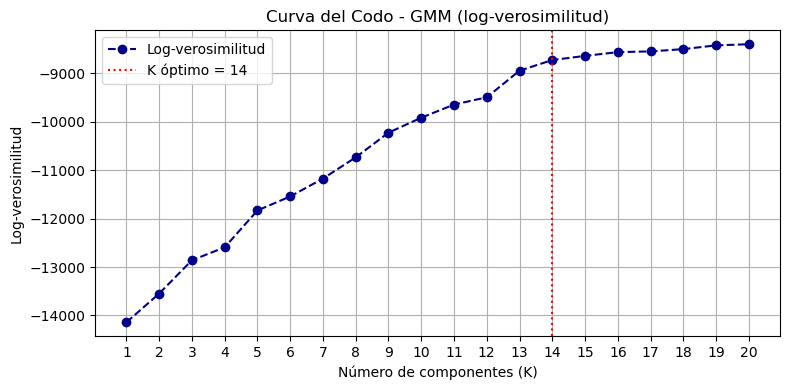
\includegraphics[width=0.6\textwidth]{figures/gmm_elbow_threshold.png}
    \caption{Curva de log-likelihood negativo en función de $K$ para GMM. Se aplicó un umbral de mejora y paciencia para detectar automáticamente el mejor valor de $K$, que resultó ser $14$.}
    \label{fig:gmm_elbow_auto}
\end{figure}

Para garantizar una buena convergencia del algoritmo EM, los parámetros iniciales del modelo GMM se tomaron a partir de los centroides y asignaciones obtenidas por K-means. Esta inicialización permitió acelerar la convergencia y evitar mínimos locales deficientes.

La Figura~\ref{fig:gmm_clusters_14} muestra la partición final obtenida para $K = 14$, donde cada color representa un componente de la mezcla. Se observa que las regiones de asignación resultan más suaves que en K-means, lo cual refleja la naturaleza probabilística del modelo.

\begin{figure}[H]
    \centering
    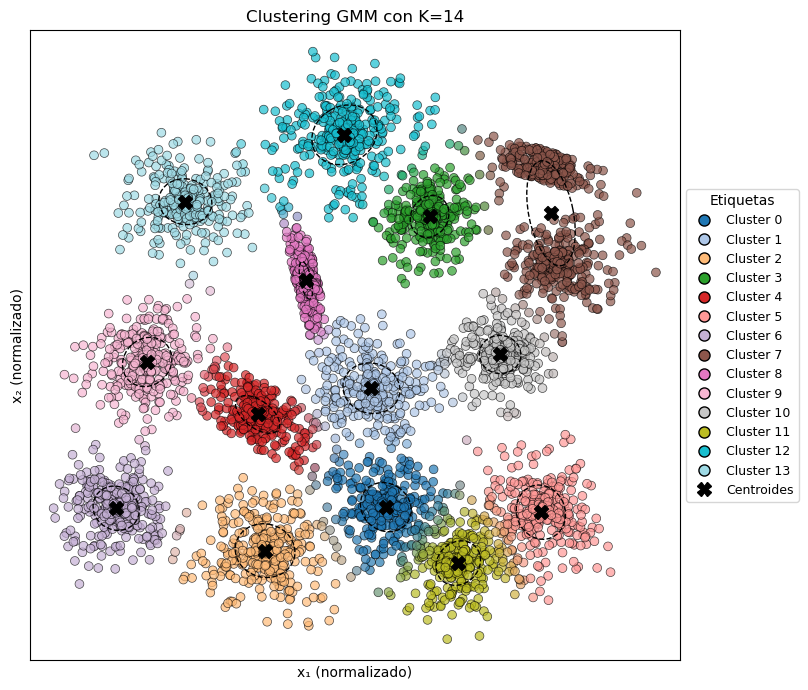
\includegraphics[width=0.6\textwidth]{figures/gmm_clusters_k14.png}
    \caption{Clusters obtenidos mediante GMM con $K = 14$. Los puntos están coloreados según el componente con mayor responsabilidad.}
    \label{fig:gmm_clusters_14}
\end{figure}

Aunque GMM tiende a captar mejor estructuras elípticas o con solapamiento, también mostró ciertas limitaciones en regiones donde las componentes gaussianas no se ajustaban perfectamente a la distribución local de los datos.


\subsection*{DBSCAN}

El algoritmo DBSCAN se aplicó con el objetivo de detectar agrupamientos basados en densidad, sin necesidad de especificar el número de clusters a priori. A diferencia de K-means y GMM, este método puede identificar regiones de forma arbitraria y distinguir ruido de estructura significativa.

DBSCAN depende de dos hiperparámetros clave:

\begin{itemize}
    \item $\varepsilon$: el radio de vecindad a considerar para cada punto.
    \item $MinPts$: la cantidad mínima de vecinos dentro de ese radio para que un punto sea considerado núcleo.
\end{itemize}

Se exploraron combinaciones de valores para $\varepsilon$ y $MinPts$, evaluando visualmente la calidad del agrupamiento y la cantidad de puntos etiquetados como ruido. El criterio de selección de la mejor configuración se basó en la coherencia de los clusters identificados, su separación y la reducción de asignaciones ambiguas.

La mejor partición se obtuvo para $\varepsilon = 0.1$ y $MinPts = 20$. Esta configuración permitió detectar con precisión las regiones densas del conjunto de datos, asignando como ruido a los puntos aislados o dispersos. La Figura~\ref{fig:dbscan_clusters} muestra el resultado final del agrupamiento.

\begin{figure}[H]
    \centering
    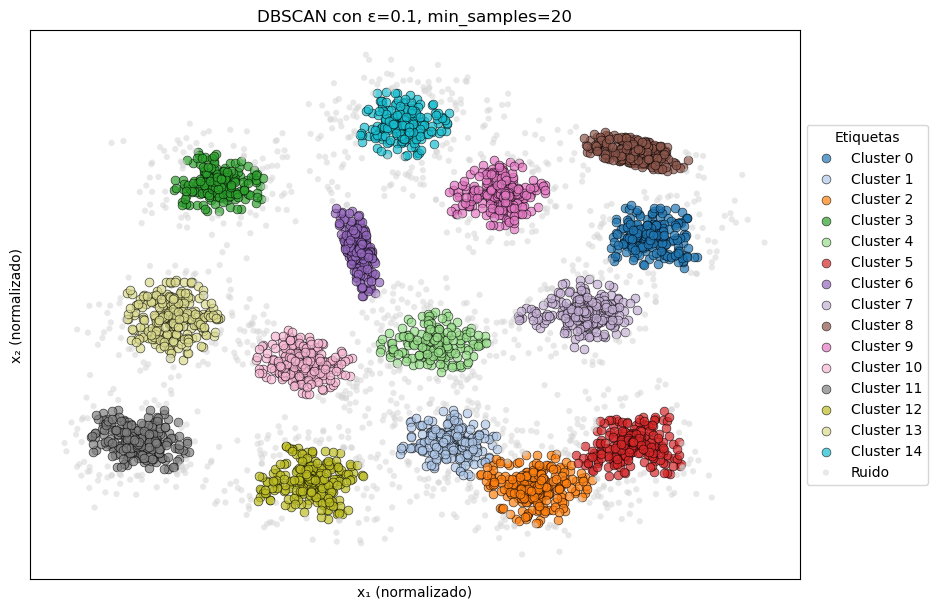
\includegraphics[width=0.6\textwidth]{figures/dbscan_clusters.png}
    \caption{Clusters obtenidos mediante DBSCAN con $\varepsilon = 0.3$ y $MinPts = 5$. Los puntos en gris corresponden a ruido (no asignados a ningún cluster).}
    \label{fig:dbscan_clusters}
\end{figure}

A diferencia de los métodos anteriores, DBSCAN logró adaptarse mejor a la forma real de los grupos presentes, separando naturalmente regiones de distinta densidad sin requerir una partición convexa del espacio. Además, resultó robusto frente a outliers, al no forzar la asignación de todos los puntos.

Este comportamiento lo posicionó como el método más efectivo para este conjunto de datos, al menos bajo criterios estructurales no paramétricos.

\section{Reducción de dimensionalidad}

Para esta parte del trabajo se utilizó el conjunto de imágenes MNIST, compuesto por dígitos manuscritos del 0 al 9 representados como vectores de dimensión $784$ ($28 \times 28$ píxeles en escala de grises). El objetivo fue obtener representaciones de menor dimensión que conserven la mayor cantidad de información posible, evaluando luego la capacidad de reconstrucción de las imágenes originales.

\subsection*{Análisis de Componentes Principales (PCA)}

Se aplicó PCA sobre el conjunto de imágenes MNIST con el objetivo de obtener representaciones comprimidas que preserven la mayor parte posible de la información original. Para ello, se analizaron dos criterios complementarios: la varianza explicada acumulada y el error cuadrático medio (ECM) de reconstrucción.

En la Figura~\ref{fig:pca_variance_plot} se muestra la varianza acumulada en función del número de componentes principales utilizadas. Se marcaron umbrales de referencia en 60\%, 70\%, 80\%, 95\% y 99\% de varianza explicada. A partir de aproximadamente $100$ componentes se alcanza mas del 90\%, lo cual sugiere que dicho valor es adecuado para capturar la estructura general de los datos sin incurrir en una pérdida significativa de información.

\begin{figure}[H]
    \centering
    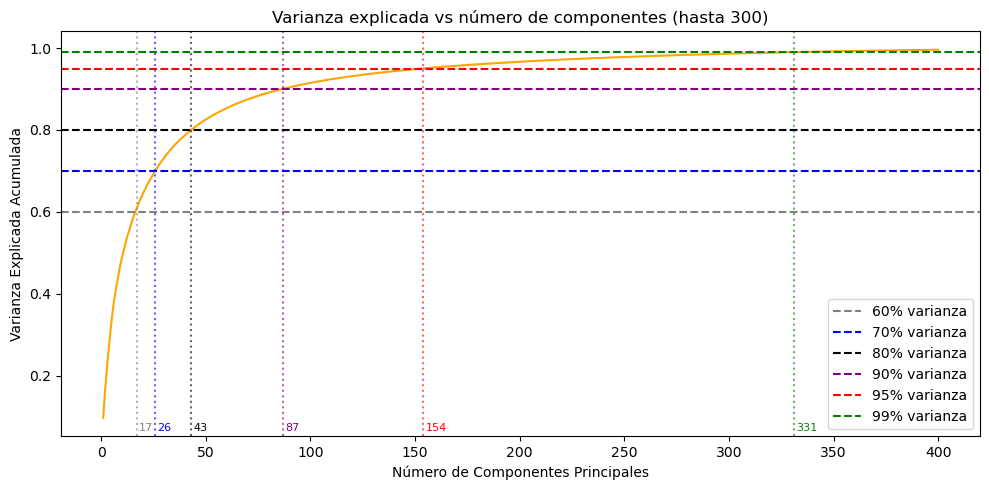
\includegraphics[width=0.65\textwidth]{figures/pca_variance_explained.png}
    \caption{Varianza explicada acumulada por PCA en función del número de componentes. Se destacan distintos umbrales de referencia.}
    \label{fig:pca_variance_plot}
\end{figure}

Por otro lado, también se calculó el error cuadrático medio de reconstrucción sobre el conjunto completo:

\[
\text{ECM}(m) = \frac{1}{n} \sum_{i=1}^{n} \|x_i - \hat{x}_i^{(m)}\|^2
\]

La Figura~\ref{fig:pca_reconstruction_error} muestra cómo varía el ECM en función de la cantidad de componentes $m$. Se observa una disminución rápida inicial, seguida de una meseta a partir de los 100 componentes, lo cual coincide con el análisis de varianza acumulada.

\begin{figure}[H]
    \centering
    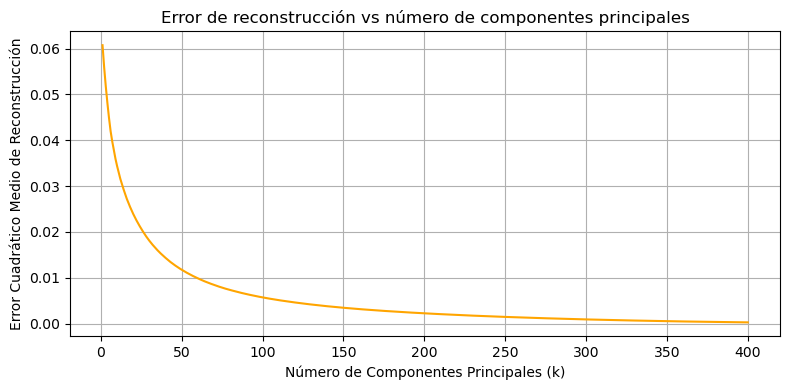
\includegraphics[width=0.65\textwidth]{figures/pca_reconstruction_error.png}
    \caption{Error cuadrático medio de reconstrucción en función de la cantidad de componentes principales.}
    \label{fig:pca_reconstruction_error}
\end{figure}

En base a ambos criterios, se seleccionaron $100$ componentes como valor de corte para la reconstrucción de imágenes. La Figura~\ref{fig:pca_reconstructed_images_100} muestra las reconstrucciones obtenidas para las primeras 10 muestras del conjunto, comparadas con sus versiones originales. Las imágenes reconstruidas mantienen adecuadamente la forma y el trazo general de los dígitos, con mínima pérdida de fidelidad visual.

\begin{figure}[H]
    \centering
    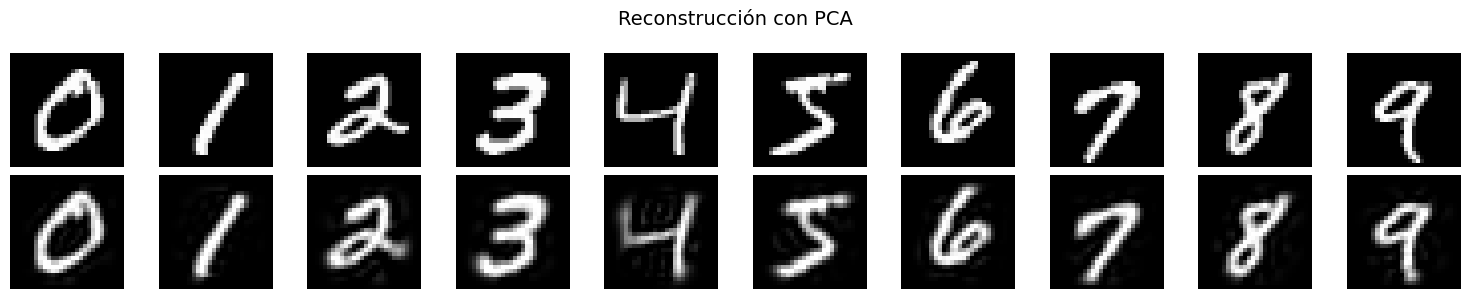
\includegraphics[width=\textwidth]{figures/pca_reconstructions_100.png}
    \caption{Reconstrucción de dígitos mediante PCA con 100 componentes principales. Fila superior: imágenes originales. Fila inferior: reconstrucciones.}
    \label{fig:pca_reconstructed_images_100}
\end{figure}

Reconstrucciones adicionales correspondientes a otros umbrales de varianza (60\%, 70\%, 80\%, 95\% y 99\%) se incluyen en el Apéndice (ver Sección~\ref{sec:appendix_pca_reconstructions}).


\subsection*{Autoencoder Variacional (VAE)}

Además del enfoque lineal basado en PCA, se entrenó un modelo de autoencoder variacional (VAE) para realizar reducción de dimensionalidad sobre el conjunto MNIST. Este modelo no lineal permite capturar representaciones latentes más expresivas, al aprender una distribución posterior aproximada $q(z \mid x)$ desde la cual se generan reconstrucciones $\hat{x}$ mediante una red decodificadora.

El conjunto de datos fue dividido en subconjuntos de entrenamiento y validación (80\%–20\%), y se entrenó el modelo minimizando la función de pérdida de evidencia inferior (ELBO), que penaliza simultáneamente la reconstrucción deficiente y el alejamiento de la distribución latente respecto al prior $\mathcal{N}(0, I)$.

Se fijó una dimensión latente de $m = 20$, y se entrenó la red durante un número fijo de épocas. En la Figura~\ref{fig:vae_reconstructed_images} se presentan las reconstrucciones obtenidas por el VAE para las mismas 10 imágenes utilizadas en el caso de PCA.

\begin{figure}[H]
    \centering
    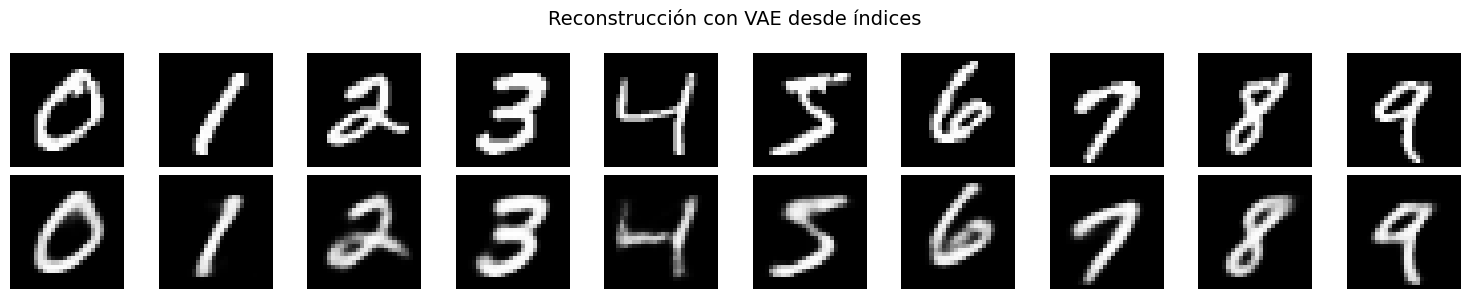
\includegraphics[width=\textwidth]{figures/vae_reconstructions.png}
    \caption{Reconstrucción de dígitos mediante VAE con dimensión latente 20. Fila superior: imágenes originales. Fila inferior: reconstrucciones.}
    \label{fig:vae_reconstructed_images}
\end{figure}

Se observa que las reconstrucciones del VAE resultan más nítidas y fieles que las obtenidas por PCA, especialmente en trazos curvos y detalles finos. La estructura general de cada dígito se conserva, y el modelo logra generar contornos más definidos y realistas.

A diferencia de PCA, que sólo captura relaciones lineales, el VAE puede aprender una transformación no lineal adaptada a la distribución de los datos. Esto le otorga mayor capacidad para comprimir la información relevante y generar representaciones latentes útiles tanto para reconstrucción como para otras tareas (por ejemplo, clasificación o generación).


\section{Conclusión}
En este trabajo se exploraron dos tareas fundamentales del aprendizaje no supervisado: el agrupamiento de datos y la reducción de dimensionalidad, utilizando métodos clásicos y modelos generativos más avanzados.

En la primera parte, se aplicaron los algoritmos K-means, Gaussian Mixture Models (GMM) y DBSCAN sobre un conjunto bidimensional. Para K-means y GMM se desarrolló una estrategia automática de selección del número de clusters basada en umbral de mejora y paciencia, resultando en $K = 15$ como valor óptimo para ambos casos. Si bien ambos métodos lograron particiones coherentes, DBSCAN fue el que mejor logró adaptarse a la estructura real de los datos sin requerir $K$ como entrada, detectando formas arbitrarias y diferenciando adecuadamente puntos ruidosos. Por este motivo, se concluye que DBSCAN fue el método más efectivo en este escenario.

En la segunda parte, se abordó la reducción de dimensionalidad sobre imágenes de dígitos manuscritos utilizando PCA y autoencoders variacionales (VAE). PCA permitió preservar más del 90\% de la varianza con 100 componentes, logrando reconstrucciones razonables. Sin embargo, el modelo VAE, con solo 20 dimensiones latentes, generó reconstrucciones de igual o mayor calidad, preservando mejor los contornos y trazos finos. Esto evidencia la capacidad superior de los modelos no lineales para capturar estructuras complejas en datos de alta dimensión.

En conjunto, los resultados muestran cómo la elección del método adecuado depende del tipo de estructura subyacente en los datos y del objetivo de la tarea. Los métodos basados en supuestos rígidos (como convexidad o linealidad) pueden ser eficientes en casos simples, pero tienden a perder capacidad expresiva frente a métodos más flexibles como DBSCAN o VAE, especialmente en contextos con formas complejas o relaciones no lineales.















\appendix
\section{Apéndice}
\subsection{Reconstrucciones adicionales con PCA}
\label{sec:appendix_pca_reconstructions}
\begin{figure}[H]
    \centering
    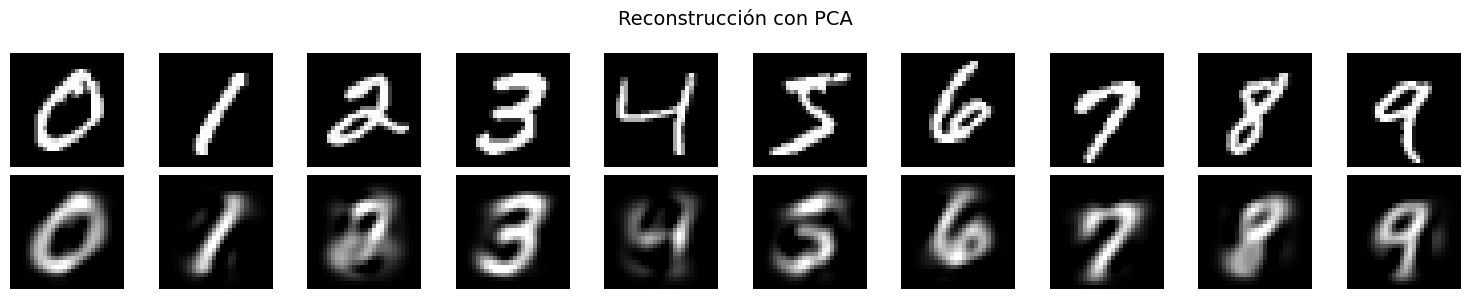
\includegraphics[width=\textwidth]{figures/pca_reconstructions_60.png}
    \caption{Reconstrucción de dígitos mediante PCA con 60\% de varianza explicada. Fila superior: imágenes originales. Fila inferior: reconstrucciones.}
    \label{fig:appendix_pca_reconstructions_80}
\end{figure}

\begin{figure}[H]
    \centering
    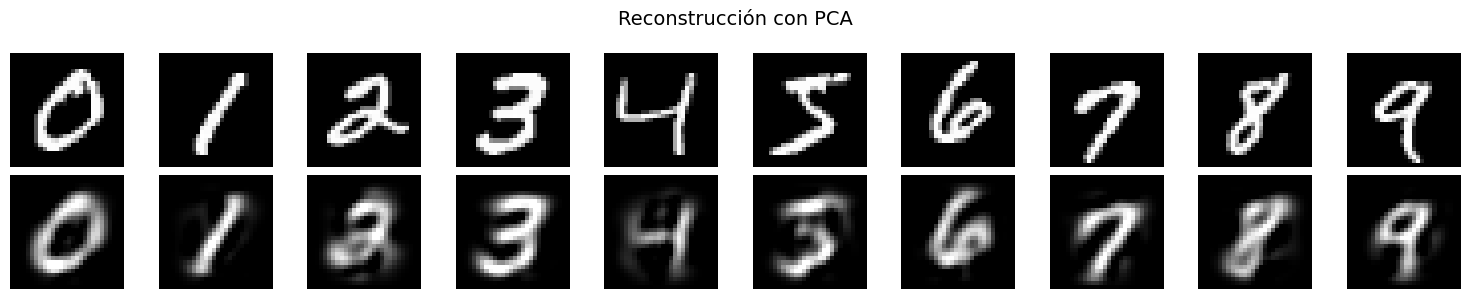
\includegraphics[width=\textwidth]{figures/pca_reconstructions_70.png}
    \caption{Reconstrucción de dígitos mediante PCA con 70\% de varianza explicada. Fila superior: imágenes originales. Fila inferior: reconstrucciones.}
    \label{fig:appendix_pca_reconstructions_70}
\end{figure}

\begin{figure}[H]
    \centering
    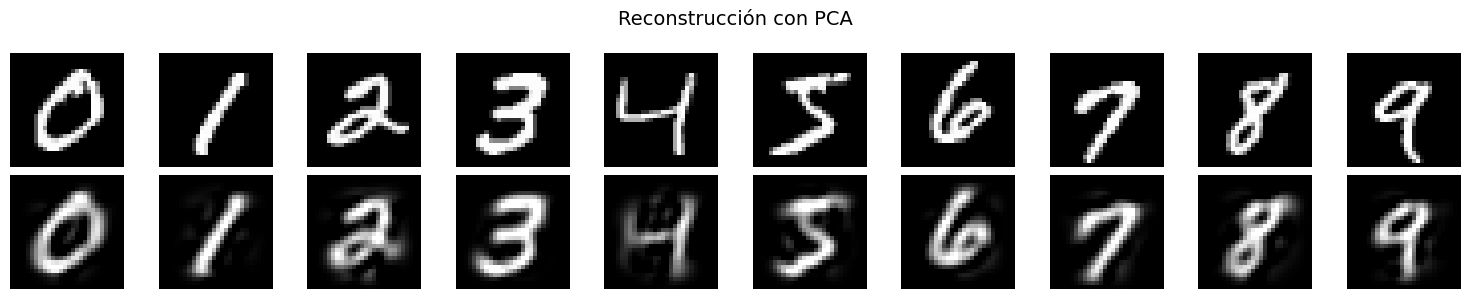
\includegraphics[width=\textwidth]{figures/pca_reconstructions_80.png}
    \caption{Reconstrucción de dígitos mediante PCA con 80\% de varianza explicada. Fila superior: imágenes originales. Fila inferior: reconstrucciones.}
    \label{fig:appendix_pca_reconstructions_80}
\end{figure}

\begin{figure}[H]
    \centering
    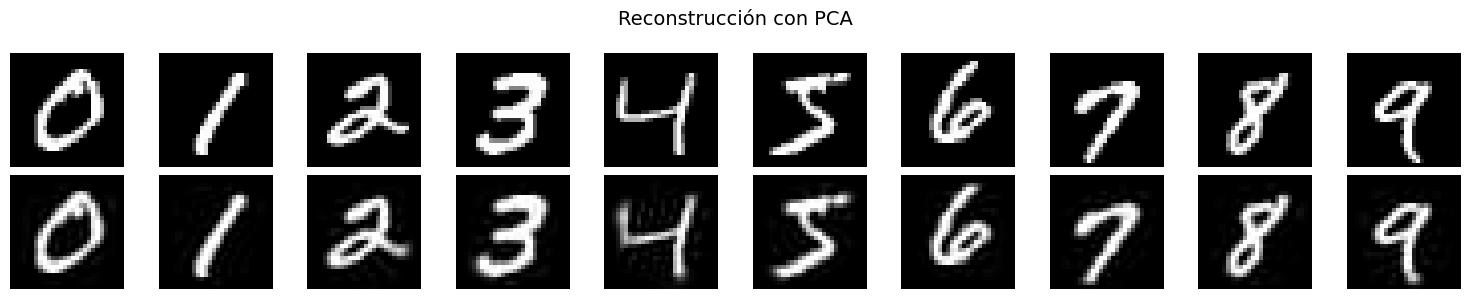
\includegraphics[width=\textwidth]{figures/pca_reconstructions_95.png}
    \caption{Reconstrucción de dígitos mediante PCA con 95\% de varianza explicada. Fila superior: imágenes originales. Fila inferior: reconstrucciones.}
    \label{fig:appendix_pca_reconstructions_95}
\end{figure}

\begin{figure}[H]
    \centering
    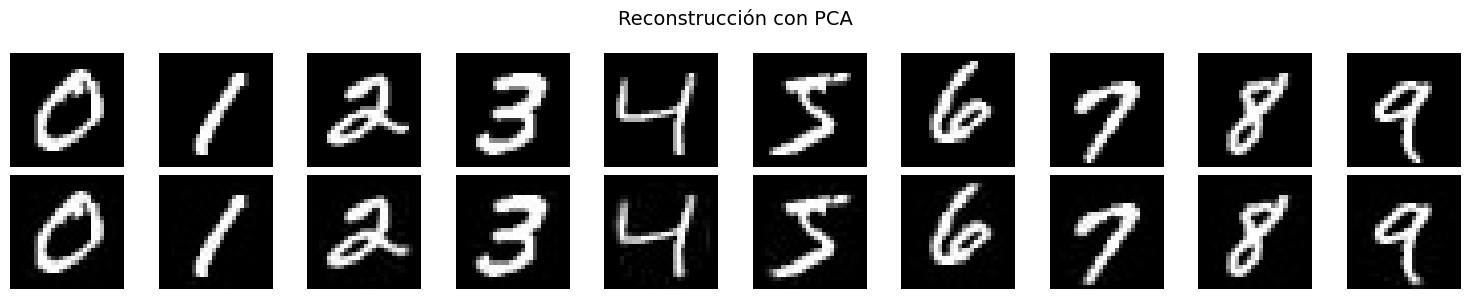
\includegraphics[width=\textwidth]{figures/pca_reconstructions_99.png}
    \caption{Reconstrucción de dígitos mediante PCA con 99\% de varianza explicada. Fila superior: imágenes originales. Fila inferior: reconstrucciones.}
    \label{fig:appendix_pca_reconstructions_99}
\end{figure}



\end{document}




